\documentclass[12pt]{article}
\usepackage{fancyvrb}
\usepackage[magyar]{babel}
\usepackage{t1enc}
\usepackage[latin2]{inputenc}
\usepackage{graphics}
\usepackage{graphicx}
\usepackage{epsfig}




\begin{document}

\section{User Manual of the refactorer}

\subsection{Installation}
\subsubsection{Windows}
We have an install tool to make it just a few click to enjoy the refactorer.
You should follow the following steps:
\begin{enumerate}
	\item Start setup.exe
	\item Choose your language (at the moment english and hungarian)
	\item Follow the instructions, read and accept the license agreement.
	\item After finishing the setup, you can try your tool by opening an .erl file in your emacs editor (do not forget, that you need a live erlang node).
\end{enumerate}


\subsubsection{Linux, MacOS, Solaris}
\begin{enumerate}
	\item First make  sure that  all  required software  components are  properly
installed and working:
\begin{enumerate}
	\item Erlang/OTP R11B (http://www.erlang.org/download.html)
  	\item GNU Emacs 21    (ftp://ftp.gnu.org/gnu/emacs/) or Aquamacs 1.1    (http://aquamacs.org/) for MacOS
  	\item MySQL 5.0       (http://dev.mysql.com/downloads/mysql/5.0.html)

\end{enumerate}

Newer versions will most probably work, older versions have not been tried.

\item Unpack the  RefactorErl release (probably you have  already done that if
you are reading this file),  we will refer to the resulting RefactorErl-VER
directory as the "base directory".
  
\item  Create a  dedicated MySQL  database for  the refactorer,  and set  up a
database user  to access it. Refer  to the MySQL documentation  to find out
details on how  to do that, but  if you don't care about  the details, here
are the commands you need to type at the MySQL command line:

  create database parse;
  grant all on parse.* to 'USER'@localhost identified by 'PASSWORD';

where  USER and  PASSWORD are  your choices  of a  username and  a suitable
password.

\item Update the  file {\tt db.config} in the base directory  using a text editor,
fill in the username and password you entered in the previous step. You may
update the name of the database as well.

\item Check the  path settings at the beginning of the  file "build.sh" in the
base directory. You need to provide the path to the base directory, and the
path of your Erlang/OTP installation.

\item Run the  script {\tt build.sh} in the base directory.  This will compile the
neccessary Erlang  modules and generates startup scripts.  After this step,
you can use  the generated script file "runerl.sh" to  start the backend of
the refatorer, and  the frontend of the refactorer will  be loaded the next
time you start Emacs.

\item  The  last  step to  complete  the  installation  is to  initialise  the
database. For this, you need to start up the refactorer:
\begin{enumerate}
	\item run {\tt runerl.sh}, which starts the backend
 	\item then start Emacs, which will load the frontend
 \end{enumerate}
 

Refactoring operations  are accessible  only for Erlang  files, so  open an
arbitrary file with .erl extension (or  create a new, empty one). Then type
{\tt C-c C-e  i} (or select Erlang->Refactor->Initialise database  in the menu)
to complete the installation. From this point, the refactorer is usable.
\end{enumerate}

\subsection{Starting the applications}

You have to start the application and initialise the database before you start to put the source code into the database.

Starting the tool is depends on your operational system:

\begin{description}
	\item[Windows systems:] You just have to start the application with {\tt runerl.bat} or just double clicking on the {\tt RefactorErl} icon.
	\item[Linux, MacOS, Solaris:] You have to \begin{itemize}
		\item run {\tt runerl.sh} which starts the backend
		\item then start Emacs, which will load the frontend
	\end{itemize}
	
\end{description}

In Emacs {\bf open the .erl} file, which you want to put into the database 
(You can find a basic Emacs tutorial in the Section \ref{emacs}, if you are not familiar with it).
If an Erlang source code is open, an Erlang menu appears in Emacs as shown in the Figure ~\ref{newmenu}.

\begin{center}
\begin{figure}[htbp]
    
    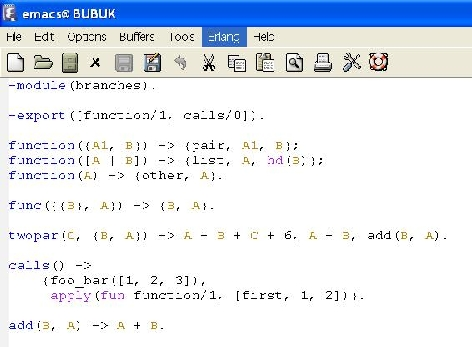
\includegraphics[scale=0.80]{newmenu.jpg}
   \caption{The Erlang menu in Emacs}
  \label{newmenu}
\end{figure}
\end{center}



\subsection{Initialise the database}

You have to choose the {\it Initialise database} command from the Erlang/Refactor menu point as shown in the Figure ~\ref{init} or use the shortcut(C-c C-e i, which means Control-c Control-e and than i (without Control) buttons).

\begin{center}
\begin{figure}[htbp]
   
    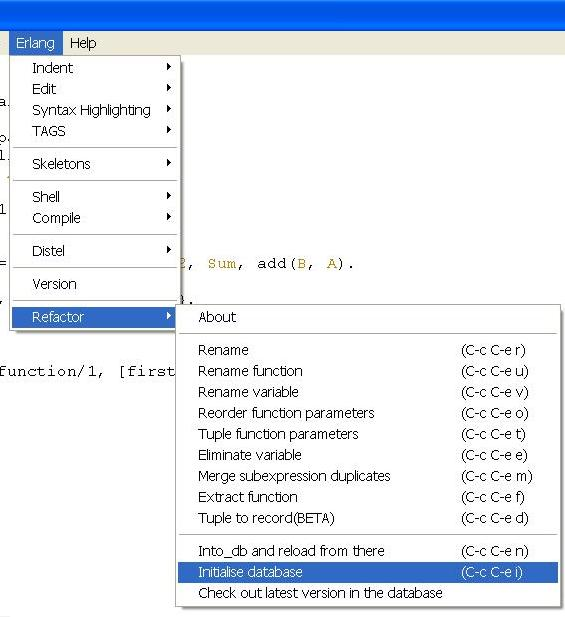
\includegraphics[scale=0.60]{init.jpg}
   \caption{Initialise the database}
  \label{init}
\end{figure}
\end{center}

When the initialisation is ready the following message appears in the minibar: *Initialised*.

\subsection{Loading the source into the database and checkout it}

After you opened the .erl file, which you want to put into the database, 
you have to choose the {\it Into\_db and reload from there} command from the Erlang/Refactor menu point as shown in the Figure ~\ref{load} 
or use the shortcut (C-c C-e n).
When the initialisation is successfully done, the following message appears in the minibar: *Reloaded*. 
In the same time the program displays the pretty-printed version of the source code in the same window.
The current file/module remains in the database until the next initialisation. 
If you put the newer version of the same file into the database, the previous version will be deleted, and  the new file will be parsed.
If you want to put more than one file into the database, you can open them and put them into the database in the same way. 
The database will contain and handle all files until the next initialisation.

\begin{center}
\begin{figure}[htbp]

    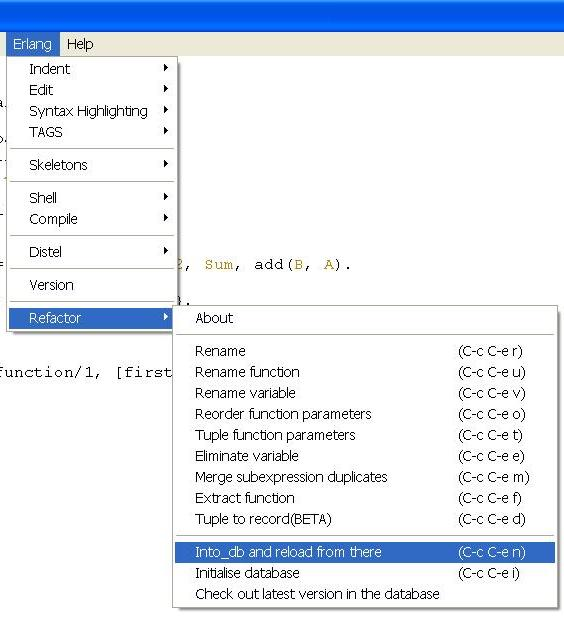
\includegraphics[scale=0.80]{load.jpg}
   \caption{Into\_db and reload from there}
  \label{load}
\end{figure}
\end{center}

If you once have put the source into the database at any time you can ask for the latest version of the source by 
choosing the {\it Check out latest version in the database} command from the Erlang/Refactor menu point as shown in the Figure ~\ref{cho}.
When the checkout is successfully done, the following message appears in the minibar: *Reloaded*. 

\begin{center}
\begin{figure}[htbp]

    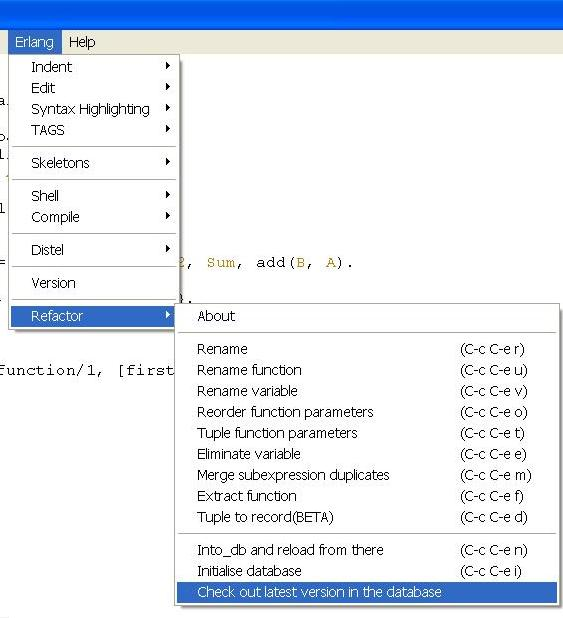
\includegraphics[scale=0.80]{checkout.jpg}
   \caption{Check out latest version in the database}
  \label{cho}
\end{figure}
\end{center}

\subsection{Executing the refactorings}

Before you want to execute a refactoring make sure, that the source is already in the database.
For example, if you previously edited the source, {\bf save} the changes and {\bf put the source into the database}.

When you are executing several refactoring after each other with no editing between them, 
you do should not put the source into the database again. 
The refactoring is executing inside the database, and just check out the source in the end.

You can start a refactoring by choosing its command from the menu or using its shortcut.
NOTE! Make sure, that you are on the needed position or you selected the needed expression(s).

For example the starting of the reorder function parameters refactoring can be seen in the Figure \ref{reorder}.

\begin{center}
\begin{figure}[htbp]

    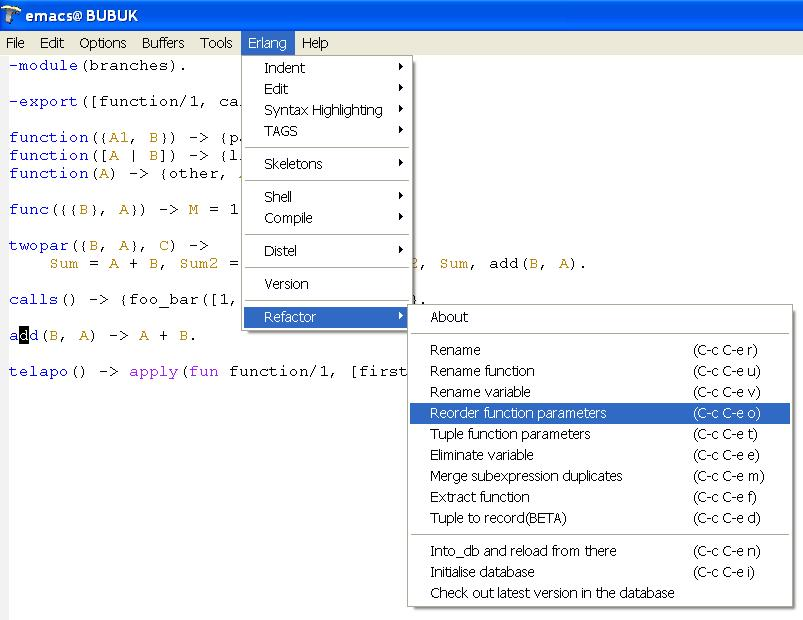
\includegraphics[scale=0.60]{reorder.jpg}
   \caption{Reorder the function parameters refactoring}
  \label{reorder}
\end{figure}
\end{center}
The result message of the refactoring can be seen in the minibar. If there is a warning, the refactoring was executed, just you get this warning.


\subsubsection{Rename variable}
\paragraph{The aim of the refactoring}
Find and rename all occurrences of the pointed variable to the new name.
\paragraph{Parameters}
You have to stand on the needed position, when you choose the refactoring from 
the menu (Rename variable or Rename) or start it with shortcut (C-c C-e r).
The other parameter will be asked during the execution in the minibar.
\begin{itemize}
	\item Position of the cursor: Somewhere inside in one occurrence of the variable.
	\item New name: The new name of the variable. 
\end{itemize}
\paragraph{Preconditions and restrictions}
The new name can not be a reserved word in Erlang, in that case the tool returns with an error message.
If the new name causes some binding problems with already existing variables in the same scope,
the tool will return with the error message and the position of the caused problem.


\subsubsection{Rename function}
\paragraph{The aim of the refactoring}
Find the definition and every call of the function and rename to the new name.
\paragraph{Parameters}
You have to stand on the needed position, when you choose the refactoring from 
the menu (Rename function or Rename) or start it with shortcut (C-c C-e r).
The other parameter will be asked during the execution in the minibar.
\begin{itemize}
	\item Position of the cursor: Somewhere inside the name of the function.
	\item New name: The new name of the function.
\end{itemize}
\paragraph{Preconditions and restrictions}
The new name has to be a legal function name (starting with capital letter and not the name of a built in Function), 
in other case the tool returns with an error message.
The new name can not cause name clash neither in the current module (existing functions, import list) 
nor in other modules, if the function is exported.

\subsubsection{Reorder function parameters}
\paragraph{The aim of the refactoring}
Change the order of the function parameters in the definition and in every call of the function
\paragraph{Parameters}
You have to stand on the needed position, when you choose the refactoring from the menu (Reorder function parameters) 
or start it with shortcut (C-c C-e o).
The other parameter will be asked during the execution in the minibar.
\begin{itemize}
	\item Position of the cursor: Somewhere inside the name of the function.
	\item New order: The new order of the parameters as a permutation of the natural numbers of 1 .. arity separated by spaces or commas.
\end{itemize}
\paragraph{Preconditions and restrictions} None

\subsubsection{Tuple function parameters}
\paragraph{The aim of the refactoring}
Change the way of using some arguments at  the definition and at 
every place of call  for a given function by grouping some arguments into one tuple argument.
\paragraph{Parameters}
You have to stand on the needed position, when you choose the refactoring from the menu (Tuple function parameters) 
or start it with shortcut (C-c C-e t).
The other parameter will be asked during the execution in the minibar.
\begin{itemize}
	\item Position of the cursor: Somewhere inside the starting parameter of the tuple
	\item Number of the tuple elements: The integer number of the new tuple's elements.
\end{itemize}
\paragraph{Preconditions and restrictions}
\begin{itemize}
	\item The given position must be within a formal argument of a function definition.
	\item The function must be a declared function, not a fun-expression.
	\item The given number must not be too large.
	\item No name clash if the arity is changing (not only in the current module if the function is exported).

\end{itemize}


\subsubsection{Eliminate variable}
\paragraph{The aim of the refactoring}
All instances of a variable are replaced with its bound value in that region where the variable is visible. 
The variable can be left out where its value is not used.

\paragraph{Parameters}
You have to stand on the needed position, when you choose the refactoring from the menu (Eliminate variable) 
or start it with shortcut (C-c C-e e).
The other parameter will be asked during the execution in the minibar.
\begin{itemize}
	\item Position of the cursor: Somewhere inside in one occurrence of the variable.
\end{itemize}
\paragraph{Preconditions and restrictions}
\begin{itemize}
	\item It has exactly one binding occurrence on the left hand side of a pattern matching expression, and not a part of a compound pattern.
	\item The expression bound to the variable has no side effects. 
	\item Every variable of the expression is visible (that is, not shadowed) at every occurrence of the variable to be eliminated. 
\end{itemize}


\subsubsection{Merge subexpression duplicates}
\paragraph{The aim of the refactoring}
The chosen expression is bound to a variable of the user's choice and all
instances of the original subexpression are changed to the variable.

\paragraph{Parameters}
You have to stand on the needed position, when you choose the refactoring from the menu or start it with shortcut.
The other parameter will be asked during the execution in the minibar.
\begin{itemize}
	\item Selected code part: it should be the extractable code part (expression or sequence of expressions).
	\item Name: the name of the new function. 
\end{itemize}
\paragraph{Preconditions and restrictions}
\begin{itemize}
\item The selected expression has to be valid.
\item The given name cannot clash with one that already exists in the given
  context and has the same scope.
\item The transformation cannot be executed of the expression is
  \begin{itemize}
  	\item in the head of list comprehension,
  	\item in a generator pattern,
  	\item in a clause guard,
  	\item in a clause pattern or
  	\item in a macro.
  \end{itemize}
  
\end{itemize}
\subsubsection{Extract function}
\paragraph{The aim of the refactoring}
An alternative of a function definition might contain an expression
(or a sequence of expressions)
which can be considered as a logical unit, hence a function definition
can be created from it. The extracted function is lifted to the module
level, and it is parameterised with the ``free'' variables of the
original expression(s): those variables which are bound outside of the
expression(s), but the value of which is used by the expression(s).
\paragraph{Parameters}
You have to stand on the needed position, when you choose the refactoring from the menu (Extract function) or start it with shortcut (C-c C-e f).
The other parameter will be asked during the execution in the minibar.
\begin{itemize}
	\item Selected code part: it should be the extractable code part (expression or sequence of expressions).
	\item Name: the name of the new function.
\end{itemize}
\paragraph{Preconditions and restrictions}
\begin{itemize}
	\item The name of the function to introduce should not conflict with another
      function, either defined in the same module, or imported from another
      module (overloading). Furthermore, the name should be a legal function name.

	\item The starting and ending positions should delimit a sequence of
      expressions. 

	\item Variables with possible binding occurrences in the selected 
      sequence of expressions should not appear outside of the 
      sequence of expressions.

	\item The extracted sequence of expressions cannot be part of a guard sequence.

	\item The extracted sequence of expressions cannot be part of a pattern.

	\item The extracted sequence of expressions cannot be part of macro definition.

	\item The extracted sequence of expressions cannot be part of a
      \newline list\_comprehension node. 

	\item If the selected sequence of expression started with brackets, you should 
      drop out these brackets.
      \end{itemize}
      
\subsubsection{Tuple to record}
\paragraph{The aim of the refactoring}
Change the same tuples in a function clause into a record. If one of the transformed tuple is in the pattern of the clause or it is the last expression of the  clause's body than function calls are affected as well. Where the transformation can not be directly applied - the transformed expression is not a tuple - conversion macros are used. Later releases will support propagation of the refactoring, therefore reducing the need of the macros.

\paragraph{Parameters}
You have to stand on the needed position, when you choose the refactoring from the menu (Tuple to record) 
or start it with shortcut (C-c C-e d).
The other parameter will be asked during the execution in the minibar.
\begin{itemize}
	\item Selected code part: should be a tuple.
	\item Record name: the name of the new record. 
	\item Record field name: the name of the new record's fields. 
\end{itemize}
\paragraph{Preconditions and restrictions}
\begin{itemize}
	\item The number of specified record fields must be equal to the number of
	elements in the selected tuple.
	\item The tuple must not be embedded into a list, or a list comprehension or into an another tuple.
	\item If you use an already exisiting record, the record field names must match the defined record
	fields. Otherwise the result will not work. Later versions will merge the new fields and the already
	existing ones.
\end{itemize}

\section{Basic Emacs tutorial}
\label{emacs}

All the basic functionality which an editor provides are available through
the File, Edit, Buffers menus' menu points:

These basic functionalities are for example
\begin{itemize}
	\item {\bf Open File}: File/Open File...
	\item {\bf Close File}: File/Close(current buffer)
	\item {\bf Quit}: File/Exit Emacs
\end{itemize}


You can select an area with a mouse, and you can make the following editings:
\begin{itemize}
	\item {\bf Copy}: Edit/Copy
	\item {\bf Cut}: Edit/Cut
	\item {\bf Paste}: Edit/Paste
\end{itemize}

{\bf Switch between opened files}: In the Buffers menu point all the currently 
 opened files are listed. Selecting one of them immediately shows that in the 
 editor.

If you are comfortable with these methods you can try to use the {\bf keyboard 
shortcut}s too:
\begin{itemize}
	\item Open File: Control-X and after that Control-F (C-x C-f)
	\item Quit: Control-X and after that Control-C (C-x C-c)

	\item Copy: Alt - W (A-w)
	\item Cut: Control - W (C-w)
	\item Paste: Control - Y (C-y)

	\item Switch between opened files:
	Control - B Switch back to the last edited file, or type in the name of the 
	 opened file (Tab auto complete is available) and press ENTER.

\end{itemize}

\end{document}

